\documentclass[tikz,border=4pt]{standalone}
\usepackage{tikz}
\usepackage{amsmath}
\usetikzlibrary{arrows.meta,calc,positioning,shapes.geometric,shapes.misc,
                backgrounds,fit,decorations.markings}

\begin{document}
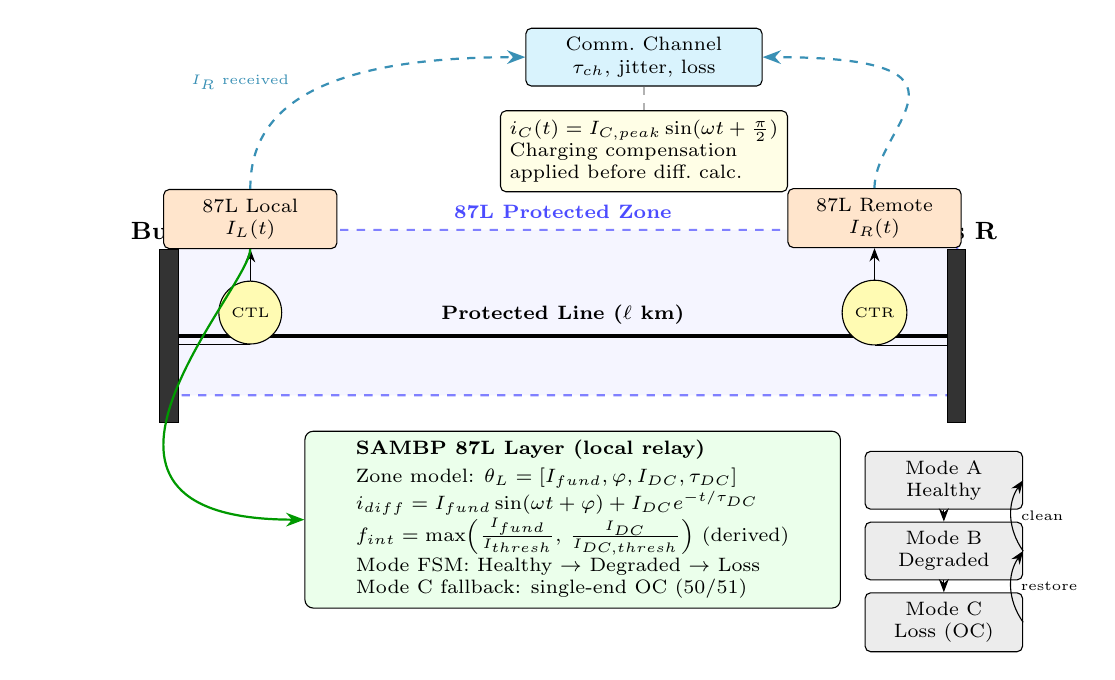
\begin{tikzpicture}[
  font=\small,
  >=Stealth,
  bus/.style   ={draw,fill=black!80,minimum width=0.12cm,minimum height=2.2cm},
  ct/.style    ={draw,circle,minimum size=0.55cm,fill=yellow!30,font=\tiny},
  relay/.style ={draw,rectangle,minimum width=2.2cm,minimum height=0.75cm,
                 fill=orange!20,align=center,font=\scriptsize,rounded corners=2pt},
  channel/.style={draw,rectangle,minimum width=3.0cm,minimum height=0.65cm,
                  fill=cyan!15,align=center,font=\scriptsize,rounded corners=2pt},
  zone/.style  ={draw=blue!50,dashed,thick,rounded corners=4pt,
                 fill=blue!4,inner sep=8pt},
  mode/.style  ={draw,rectangle,minimum width=2.0cm,minimum height=0.55cm,
                 fill=gray!15,align=center,font=\scriptsize,rounded corners=2pt},
]

%% ============================================================
%%  Bus bars (local = left, remote = right)
%% ============================================================
\node[bus,label=above:\textbf{Bus L}] (busL) at (0,0)   {};
\node[bus,label=above:\textbf{Bus R}] (busR) at (10,0)  {};

%% Line conductor
\draw[ultra thick] (busL.east) -- node[above,font=\scriptsize\bfseries]
      {Protected Line ($\ell$ km)} (busR.west);

%% ============================================================
%%  Local end: CT + relay
%% ============================================================
\node[ct,right=0.5cm of busL.east,yshift=0.3cm] (ctL) {CT\\L};
\draw (busL.east |- ctL.south) -- (ctL.south);
\node[relay,above=0.4cm of ctL] (relayL)
      {87L Local\\$I_L(t)$};
\draw[->] (ctL.north) -- (relayL.south);

%% ============================================================
%%  Remote end: CT + relay
%% ============================================================
\node[ct,left=0.5cm of busR.west,yshift=0.3cm] (ctR) {CT\\R};
\draw (busR.west |- ctR.south) -- (ctR.south);
\node[relay,above=0.4cm of ctR] (relayR)
      {87L Remote\\$I_R(t)$};
\draw[->] (ctR.north) -- (relayR.south);

%% ============================================================
%%  Communication channel
%% ============================================================
\node[channel,above=1.3cm of relayL,xshift=5cm] (chan)
      {Comm.\ Channel\\$\tau_{ch}$, jitter, loss};
\draw[->,dashed,cyan!70!black,thick]
      (relayL.north) .. controls +(0,0.8) and +(-3,0)
      .. node[above left,font=\tiny]{$I_R$ received} (chan.west);
\draw[->,dashed,cyan!70!black,thick]
      (relayR.north) .. controls +(0,0.8) and +(3,0)
      .. (chan.east);

%% ============================================================
%%  SAMBP block (centred below line)
%% ============================================================
\node[draw,fill=green!8,rounded corners=3pt,
      below=1.2cm of busL.east,xshift=5cm,align=left,
      font=\scriptsize,minimum width=6.8cm] (sambp)
      {\textbf{SAMBP 87L Layer (local relay)}\\[2pt]
       Zone model: $\theta_L=[I_{fund},\varphi,I_{DC},\tau_{DC}]$\\
       $i_{diff}=I_{fund}\sin(\omega t+\varphi)+I_{DC}e^{-t/\tau_{DC}}$\\
       $f_{int}=\max\!\left(\tfrac{I_{fund}}{I_{thresh}},\,
                             \tfrac{I_{DC}}{I_{DC,thresh}}\right)$ (derived)\\
       Mode FSM: Healthy $\to$ Degraded $\to$ Loss\\
       Mode C fallback: single-end OC (50/51)};

\draw[->,thick,green!60!black]
      (relayL.south) .. controls +(0,-0.5) and +(-3.5,0)
      .. (sambp.west);

%% ============================================================
%%  Mode state boxes
%% ============================================================
\node[mode,right=0.3cm of sambp,yshift=0.5cm]  (mA) {Mode A\\Healthy};
\node[mode,below=0.15cm of mA]                  (mB) {Mode B\\Degraded};
\node[mode,below=0.15cm of mB]                  (mC) {Mode C\\Loss (OC)};
\draw[->] (mA.south) -- (mB.north);
\draw[->] (mB.south) -- (mC.north);
\draw[->,bend left=35] (mC.east) to node[right,font=\tiny]{restore} (mB.east);
\draw[->,bend left=35] (mB.east) to node[right,font=\tiny]{clean} (mA.east);

%% ============================================================
%%  Zone boundary
%% ============================================================
\begin{scope}[on background layer]
  \node[zone,fit=(ctL)(ctR),inner sep=18pt,
        label={[font=\scriptsize\bfseries,blue!70]above:87L Protected Zone}] {};
\end{scope}

%% ============================================================
%%  Charging current annotation
%% ============================================================
\node[draw,fill=yellow!10,rounded corners=2pt,
      below=0.3cm of chan,align=left,font=\scriptsize,
      minimum width=3.0cm] (iC)
      {$i_C(t)=I_{C,peak}\sin(\omega t+\tfrac{\pi}{2})$\\
       Charging compensation\\
       applied before diff.\ calc.};
\draw[dashed,gray!60] (chan.south) -- (iC.north);

\end{tikzpicture}
\end{document}
